
%3/4 pages au moins en français (idem pour conclusion)
%\begin{itemize}
%\item fines échelles et leur rétroaction/structuration de circu générale
%\item choix région Gibraltar (Rencontre deux masses d'eaux, alimentation MédiTerranée, outflow med)
%\item les fines échelles à Gibraltar (quels phénomènes (solitons, ressaut, etc))
%\item Outils de la thèse : num, obs (compagne,sat)
%\item état des lieux modélisation num fines échelles océaniques, problematique quantification mélange diapycnale
%\item plan
%\end{itemize}

%Certains des éléments bibliographiques sont repris dans les introductions des différents chapitres, conçus comme des articles.

\section[Un voyage en \textit{Terra Incognita}]{Un voyage en \textit{Terra Incognita\footnote{\cite{scotti_large_2010}}}}
\subsection{Dynamique océanique : vers les fines échelles}
\label{subsection_intro1}
%(pose principes circu océanique, présente contexte des échelles généralement considérées en océanographie physique)

%La circulation globale océanique, pilotée par les vents et le flux de flottabilité, s'organise en un ensemble de courants de grande échelles (gyre, AMOC,...) qui en parallèle et en interaction avec la dynamique de l'atmosphère, transporte la chaleur. \\


La dynamique de l'océan est variée, et le \textit{spectre} des processus qui composent cette dynamique s'étend sur une large gamme autant spatiale que temporelle. La houle, les courants d'Ekman, les systèmes d'upwelling ou de downwelling, les ondes de marée, les marées internes, la convection profonde, les courants de gravité ou encore les panaches fluviaux, en représentent une fraction. Ces processus constituent la réponse de l'océan, vu comme un \textit{système dynamiquement ouvert} à un ensemble de forçages externes : la pression atmosphérique à sa surface, les marées astronomiques, des flux de quantité de mouvement induits par le vent, flux de chaleur radiatifs, ou flux de matière par les précipitations, les fleuves ou encore par évaporation, \textit{et cetera}...

Mais l'océan ne se résume toutefois pas à une somme de processus "forcés" dont la combinaison linéaire suffirait à expliquer sa dynamique propre. Ces processus interagissent  entre eux induisant d'importants \textit {mécanismes de transferts} de propriétés physiques (ie, sous forme d'énergie) et dynamiques (ie, la vorticité) entre les différentes gammes d'échelles spatiales et temporelles du spectre. Ces mécanismes sont en partie évoqués ci-après et schématisés dans la figure \ref{fig_ocean_scales}. 

Lorsque les transferts prennent spatialement et temporellement une forme cohérente, on parle de \textit{cascades d'échelles} ou de \textit{cascades turbulentes} \citep{lapeyre_topologie_2000}. Les mécanismes débouchant sur ces transferts sont, quant à eux, généralement associés à des \textit{instabilités dynamiques} dont la nature va varier d'une région du spectre spatio-temporelle à l'autre, en particulier car l'effet de la rotation de la Terre sur leur développement n'est pas pris en compte de la même façon selon la taille des structures impliquées.

Ainsi, à méso-échelle \footnote{Région du spectre constitué d'échelles plus grandes que le premier rayon de Rossby, $Ro$, de l'ordre de la dizaine voir de la centaine de kilomètres.} (région 1 de la figure \noparref{fig_ocean_scales}), la stratification de la colonne d'eau et la rotation du globe terrestre jouent tous deux des rôles prépondérants et peuvent localement être associées à des équations de bilan de quantité de mouvement équilibrées. Ainsi, par exemple, l'action de la rotation de la Terre peut donner à l'océan un comportement de colonnes de Taylor.

\begin{figure}[!h]
  \centering
  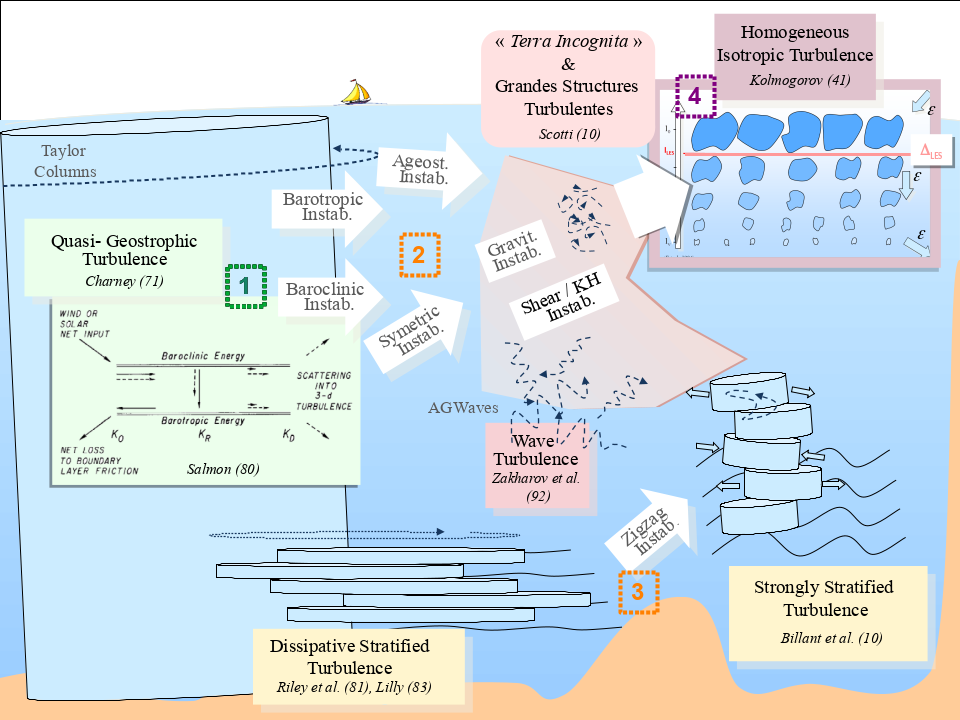
\includegraphics[width=0.8\textwidth]{./INTRO/Ocean_Scales.png}
  \caption{L'océan vu à travers ses cascades d'échelles, ses instabilités et ses principaux modèles de turbulence. (1) La méso-échelle. (2) et (3) la sous-mésoéchelle. (4) la micro-échelle. $\Delta_{LES}$ est l'échelle juste en-deçà des grandes structures turbulentes. D'après \citet{charney_geostrophic_1971, salmon_baroclinic_1980,riley_direct_1981,lilly_stratified_1983,zakharov_wave_1992,billant_zigzag_2010,kolmogorov_local_1941,scotti_large_2010}.}
  \label{fig_ocean_scales}
\end{figure}
\citep{}
A cette échelle, \citet{charney_geostrophic_1971} parle de régime de \textit{turbulence géostrophique} (ou quasi-géostrophique) qui met en jeu instabilités \textit{barotropes}\footnote{Littéralement "qui ne dépend que de la pression", i.e. dont les surfaces isopycnales sont confondues avec les surfaces isobares.} et \textit{baroclines}\footnote{Qui ne sont pas barotropes}. \cite{salmon_baroclinic_1980} montre que les transferts s'organisent de façon cohérente sous la forme d'une \textit{cascade inverse} associée à des transferts énergétiques barotropes dirigés majoritairement vers de plus grandes échelles dites synoptiques\footnote{Une telle cascade "inverse" est caractéristique de régimes de turbulence 2D.}. Les transferts d'enstrophie\footnote{A l'image de l'énergie cinétique pour la vitesse, l'enstrophie est définie comme la moitié du carré de la vorticité relative, i.e. du rotationnel de la vitesse.} sont quant à eux majoritairement dirigés vers de plus fines échelles. La cascade inverse demeure toutefois un modèle qualitatif fournissant une grille de lecture pour les processus complexes et "non localisés" du spectre océanique.

%Par exemple des structures dynamiques baroclines\footnote{Qui ne sont pas barotropes} de méso-échelles issus du forçage par les vents et/ou flux de chaleur se brisent lorsque l'écoulement devient instable \citep{vallis_atmospheric_2006}.

%Les vents et les flux de chaleur induisent ainsi des structures dynamiques (baroclines\footnote{Qui ne sont pas barotropes}) qui sont brisées lorsque l'écoulement devient instable \citep{vallis_atmospheric_2006}.

%Les \textit{instabilités barotropes et baroclines\footnote{Qui ne sont pas barotropes}} sont au coeur de cette \textit{cascade dite inverse}\color{red}(sur le schéma plutît cascade vers petites echelles)\color{black}, elles rythment les transferts autour des rayons de Rossby barotropes et baroclines\footnote{Échelles caractéristique de longueur caractérisant localement l'impact de la rotation du globe terrestre sur une colonne océanique de stratification donnée.} dans les écoulements de mésoéchelles. On parle de régime de \textit{turbulence géostrophique} (ou quasi-géostrophique) \citep{charney_geostrophic_1971} dans une région du spectre où stratification de la colonne d'eau et rotation du globe terrestre jouent toutes les deux des rôles prépondérants et peuvent localement être associées à des équations de bilan de quantité de mouvement équilibrées. La cascade inverse demeure toutefois un modèle qualitatif fournissant une grille de lecture pour les processus complexes et "non localisés" du spectre océanique.

Dans la gamme d'échelles spatio-temporelles inférieures, les structures dites de \textit{sous- mésoéchelle} (région 2 sur la figure \noparref{fig_ocean_scales}) sont elles aussi sujettes à un large éventail d'instabilités \citep{mcwilliams_submesoscale_2016}: instabilité agéostophique, symétrique, frontale, convective, ou encore instabilités de cisaillement, instabilités baroclines dans la couche de mélange océanique, instabilités paramétriques des ondes internes... Dans cette région du spectre, l'impact de la rotation du globe terrestre est plus faible qu'à mésoéchelle mais la stratification contraint fortement la dynamique océanique, débouchant sur des formes de turbulence dites "stratifiées" (région 3 de la figure \noparref{fig_ocean_scales}): la \textit{turbulence stratifiée dissipative}, la \textit{turbulence fortement stratifiée} \citep{augier_turbulence_2012}, avec l'instabilité "zig-zag" faisant office de pont entre ces deux formes de turbulence \citep{billant_zigzag_2010}.

En deçà de cette sous-mésoéchelle (on parle de \textit{microéchelle}, région 4 de la figure \noparref{fig_ocean_scales}), une autre cascade présentant elle-aussi une certaine cohérence peut prendre naissance : la \textit{cascade directe} ou cascade de Richardson. Là, l'énergie est transférée "directement" vers l'échelle de Kolmogorov au-delà de laquelle la dissipation moléculaire est majoritairement active. Si les théories décrivant les transferts à mésoéchelle ne s'accordent pas à montrer de routes directes vers la dissipation, les transferts depuis la sous-mésoéchelle le permettent, mais de façon locale et intermittente.

En parallèle de cette route depuis la sous-mésoéchelle, la micro-échelle émerge aussi de la propagation en continue des ondes de gravité internes et des ondes de gravité de surface dans l'océan. L'interaction de ces nombreuses ondes donne lieu à une forme particulière de turbulence, appelée \textit{la turbulence d'onde}. Le déferlement de ces ondes, leurs instabilités donnent généralement naissance à des "patchs turbulents" intermittents annoncés par l'apparition de grandes structures turbulentes.

%Les myriades d'ondes de gravité internes et d'ondes de gravité de surface interagissent aussi au point de donner lieu à une forme particulière de turbulence: \textit{la turbulence d'onde}. Leur déferlement, leurs instabilités donnent généralement naissance à des "patchs turbulents" intermittents annoncés par l'apparition de grandes structures turbulentes.

Ces \textit{grandes structures turbulentes} marquent en effet l'entrée de la cascade directe, elles sont associées à des instabilités de cisaillement telles que les instabilités de Kelvin-Helmholtz. Le reste de la cascade directe à micro-échelle est ensuite décrit par un modèle de turbulence homogène et isotrope 3D. Mais comme les mécanismes entraînant ces instabilités de cisaillement vont être variés les échelles spatiales et temporelles des grandes structures turbulentes ne sont pas clairement définies : elles peuvent atteindre quelques dizaines de mètres au sein de la colonne d'eau (cisaillement au bord d'un courant) mais peuvent aussi ne pas dépasser le mètre dans les couches de surface ou de fond (cisaillement de couches limite).

Cascades d'échelles et modèles de turbulence décrivent ainsi des régions spécifiques du spectre spatio-temporel de l'océan présentant une certaine cohérence. Les instabilités dynamiques tissent quant à elles des ponts entre ces régions. En toute rigueur, comprendre, expliquer, \textit{simuler} (explicitement) ou \textit{modéliser} (implicitement) le mélange turbulent, implique donc évidemment de représenter correctement l'ensemble du spectre océanique, ses transferts, ses cascades... La cascade turbulente directe, i.e. le transfert "inertiel" d'énergie aboutissant à la région "dissipative" du spectre doit faire l'objet d'un soin tout particulier. Le point d'origine de cette cascade au sein du spectre océanique n'est cependant pas clairement défini et la localisation physique de cette cascade varie aussi bien dans le temps que dans l'espace. Seule l'apparition souvent intermittente de grandes structures turbulentes semble permettre de localiser spatialement et temporellement ce point de départ.
%Les grandes structures turbulentes marquent donc l'entrée de la cascade directe menant à la dissipation moléculaire. Elles sont ainsi à l'origine d'une cascade débouchant sur une réorganisation irréversible, diabatique de la colonne d'eau et d'un redistribution des "traceurs" passifs ou actifs. Parmi ces "traceurs", la masse volumique joue un rôle particulier dans la dynamique océanique: les masses d'eau sont par exemple "transportées" le long des surfaces isopycnales et le contenu en vorticité potentielle entre deux de ces surfaces isopycnales se conserve au cours du temps.\\

A. Scotti \citep{scotti_large_2010}, dans une revue sur la modélisation de l'océan, conclut qu’avec l'étude des grandes structures turbulentes, s'ouvrent les portes de la \textit{Terra Incognita}. Il reprend ainsi la conclusion de J.C. Wyngaard \citep{wyngaard_toward_2004} rédigée quelques années auparavant pour l'atmosphère. Cette terre inconnue, souvent aussi qualifiée de "zone grise" abritant les \textit{fines échelles océaniques}, est plus largement considérée comme la région particulièrement mal connue du spectre océanique dans laquelle la dynamique peut localement et temporairement basculer d'un équilibre simple entre un nombre limité de processus à une dynamique non-linéaire complexe induisant une cascade (directe) d'instabilités dynamiques aboutissant à la dissipation moléculaire. 
\color{black}
%Cependant, l'océan (tout comme l'atmosphère) a un écoulement turbulent, c'est-à-dire chaotique et non-linéaire/ constitué d'une intéraction d'échelle.
%...
%Cette turbulence se manifeste en la décomposition des structures de grande échelles/synoptiques en des champs de plus petite structures/structures de plus en plus petites (transiant?) en intéractions les unes avec les autres (tourbillons, etc). Ainsi l'étude de l'océan peut se faire à bien des échelles spatiales et temporelles
%Ce manuscrit de thèse porte sur l'étude d'une dynamique dite de 'fine échelle', sur les processus / phénomènes océaniques . Il s'agira 
%\color{blue}
\subsection{Mélange et rétroactions}
\label{subsection_retroactions}

A l'aboutissement de ces transferts et cascades d'échelles, la dissipation moléculaire va modifier les propriétés du fluide océan, c'est le mélange.
%Le mélange  issu des processus de dissipation peut ainsi être présenté comme l'aboutissement de transferts et de cascades plus ou moins cohérents mais quoiqu'il en soit très hétérogènes et intermittentes. 
Il ne constitue toutefois pas un puits sans fond ou un aller sans retour. Les flux diapycnaux\footnote{normal aux surfaces isopycnales} modifient en effet les propriétés thermo-halines des masses d'eau, et la dissipation visqueuse près du fond "injecte" de la vorticité potentielle\footnote{La vorticité potentielle est une quantité, une substance d'après \cite{haynes_conservation_1990}, essentielle dans la description des écoulements stratifiés en rotation qui est conservée par advection}. L'accumulation de telles modifications va \textit{in fine} se répercuter sur la réponse de l'océan à ses forçages et sont donc autant d'exemples de rétroactions sur la grande échelle.
%\color{red}(grandes srtructure sturbulentes, couvre large gamme d'échelle, point vocab si est dans fine échelle/sous-mésoéchelle ou micro échelle...., selon où est LES zonale... Je ne suis pas sûr de comprendre ta remarque, on en rediscute ce matin si tu veux. Francis)\color{blue}\\


%La région du détroit de Gibraltar séparant la mer Méditerranée de l'océan Atlantique est à ce titre tout à fait exemplaire. Les masses d'eau méditerranéennes et atlantiques s'y croisent de façon éphémère et brutale. Le mélange induit par les fortes amplitudes de marée de ces deux masses d'eau  modifie in fine salinité et quantité de mouvement de ces masses d'eau. Il exerce donc un contrôle sur la dynamique de l'ensemble de la mer Méditerranée \citep{FA1988}, scellant en quelques sortes le régime dynamique de l'ensemble de ce bassin et fixant vraisemblablement le contenu en vorticité potentielle du jet méditerranéen en Atlantique Nord.

La région du détroit de Gibraltar séparant la mer Méditerranée de l'océan Atlantique est à ce titre tout à fait exemplaire. Il s'agit d'un point de passage entre les deux bassins; c'est en particulier le point d'entrée de la majorité des eaux qui circulent en Méditerranée, et l'origine de la masse d'eaux méditerranéennes participant à la circulation dans le bassin nord atlantique. Comme indiqué dans le paragraphe suivant, le croisement d'eaux atlantiques et méditerranéennes dans une région géographiquement limitée et à forte amplitude de marée induit un mélange qui va modifier in fine salinité et quantité de mouvement de ces masses d'eau. Il exerce donc un contrôle sur la dynamique de l'ensemble de la mer Méditerranée \citep{FA1988}, décidant en quelque sorte le régime dynamique de l'ensemble de ce bassin et fixant vraisemblablement le contenu en vorticité potentielle de la veine méditerranéenne en Atlantique Nord.\\


La dissipation turbulente exerce donc une rétroaction sur les plus grandes échelles du spectre océanique : elle  structure les masses d'eau mais aussi la circulation océanique.
\color{black}
%(Revient plus en détail sur la turbulence, cas où mot est utilisé (turbulence géostrophique? vs cascade turbulente))
%Turbulence de mésoéchelle (instabilité barocline), ici on s'intéresse au début de la cascade turbulente directe définie par Kolmogorov. Les 2 sont similaires en ce qu'elles concernent le transfert d'énergie vers de plus fines échelles. Pour le cas de la turbulence de fine échelle, // mais va aussi aboutir à structuration de l'écoulement en lui-même. (La conservation de la vorticité potentielle (PV) peut agir comme un effet structurant de jet/courants...//méandres d'un jet / courant structurés par la conservation de la vorticité potentielle... PV générée par diabatic processes (in boundary layers?)...

%Cascade inverse???

\subsection{Le détroit de Gibraltar}

Les talus continentaux, dorsales océaniques, monts sous-marins isolés et autres détroits sont autant d'accidents bathymétriques qui canalisent, perturbent, modifient la circulation générale des masses d'eau océaniques et plus généralement la dynamique de l'océan. Les accidents bathymétriques sont localement le siège de régimes de couches limites particuliers entraînant quasi-systématiquement l'apparition de structures turbulentes très localisées spatialement et ouvrant ainsi les portes de la "Terra Incognita".

Le détroit de Gibraltar a déjà été cité dans le paragraphe précédent (\S \noparref{subsection_retroactions}) comme exemple de région abritant des processus de fines échelles structurant la dynamique océanique de grande échelle. Il constitue l'archétype de l'accident topographique contraignant fortement la dynamique océanique. Le détroit est en effet la seule connexion de la mer Méditerranée à l'océan global. Ses dimensions spatiales sont réduites sur la verticale (de 300 m à 1 km de profondeur seulement) et sur l'horizontale (de l'ordre de la quinzaine de kilomètres entre les côtes marocaines et espagnoles). L'échange de masses d'eaux entrantes et sortantes, dit \textit{échange barocline}, entre les deux bassins méditerranéen et nord-atlantiques est ainsi canalisé. Le croisement de ces deux flux donne un transport net barotrope qui, en moyenne temporelle, est positif pour la Méditerranée et compense l'évaporation annuelle dans ce bassin \citep{Bryden94}.

La circulation dans le détroit à l'échelle locale ne se résume cependant pas à l'alimentation de la Méditerranée. L'accélération des courants par effet de canalisation par la bathymétrie et les côtes se cumule au courants induits par la marée semi-diurne pour engendrer des courants relativement élevés (de l'ordre de ou dépassant le $m/s$) qui vont évoluer à l'échelle de l'heure (voire de la demi-heure). En particulier, les courants peuvent être suffisamment élevés pour dépasser la vitesse de propagation de certaines ondes internes de gravité : on dit alors que le \textit{flot est surcritique} \citep{Baines1995}. La canalisation par la côte et la bathymétrie variant sur de courtes distances, le flot peut passer localement d'un régime sur-critique à sous-critique en modifiant les conditions d'écoulement des eaux atlantiques et méditerranéennes. Au niveau du seuil principal du détroit de Gibraltar, le seuil de Camarinal, une telle transition entraîne la formation puis la relaxation d'un \textit{ressaut hydraulique interne} au cours du cycle de marée \citep{FA1988}.

Le seuil de Camarinal est l'accident bathymétrique le moins profond du détroit et se présente comme une véritable barrière que les eaux méditerranéennes qui circulent sous les eaux atlantiques doivent franchir. Une fois franchis cet obstacle, les eaux méditerranéennes s'écoulent vers l'ouest comme un \textit{courant de gravité}. A cet écoulement s'ajoute la dynamique du \textit{ressaut hydraulique interne}, provoquant un mélange fort, local et intermittent des eaux méditerranéennes et atlantiques \citep{wesson_1994,GarciaLafuente2011}.

La relaxation du ressaut hydraulique interne qui a lieu lors de la renverse de marée se fait de surcroît sous la forme d'une onde interne de très grande amplitude qui se propage vers la Méditerranée en évoluant en solibore puis en un train d'ondes solitaires (ou solitons). Ces structures de grande amplitude sont elles-mêmes associées à une augmentation locale du mélange pendant leur propagation mais aussi et surtout lors de leur déferlement \citep{vlasenko_2009}. \\

La dissipation turbulente est répartie de façon très hétérogène dans la colonne d'eau océanique, souvent préférentiellement dans les couches de surface et de fond et généralement sous la forme d'événements intermittents (on parle de bouffées turbulentes). Ces caractéristiques compliquent grandement sa localisation et sa quantification même si son impact sur la circulation générale est maintenant reconnu et décrit de façon très qualitative \citep{de_lavergne_abyssal_2017}. 
La région du détroit de Gibraltar offre cependant un terrain d'étude particulièrement pertinent pour qui souhaite explorer cette dissipation turbulente et ses rétroactions. En effet les bouffées turbulentes semblent être associées aux régimes dynamiques présentant de fortes amplitudes de marée (donc facilement localisables dans le temps) et être préférentiellement localisées au-dessus des principaux seuils parsemant le détroit (facilement localisables géographiquement et relativement peu profonds).

Le choix du détroit de Gibraltar comme région d'étude privilégiée pour mes travaux de doctorat se justifie donc à plusieurs titres. Elle est particulièrement adaptée pour une première exploration en \textit{Terra Incognita} puisque les portes ouvrant une voie vers cette terre inconnue semblent y être facilement localisables : des structures turbulentes "intenses" peuvent être plus facilement observables au sein de la colonne d'eau et simulées numériquement de façon explicite. Le détroit de Gibraltar est de plus une région de choix pour mieux appréhender l'impact (la rétroaction) que pourrait imposer la dissipation turbulente sur la circulation générale dans les bassins méditerranéen et nord-atlantique: il s'agit donc d'une région privilégiée pour étudier comment cette dissipation peut structurer la dynamique océanique à beaucoup plus grande échelle.


\section{Une exploration des fines échelles océaniques}
%\color{red}
%(verrous puis objectif)
\subsection{Définir les fines échelles océaniques}
Objet central de mes travaux de doctorat, les \textit{fines échelles} océaniques doivent en premier lieu être clairement définies. Jusqu'ici, ces fines échelles ont plus spécifiquement été associées dans notre introduction (\S \noparref{subsection_intro1}) à la région du spectre océanique identifiée comme \textit{Terra Incognita}.\\

\noindent\fcolorbox{lightgray}{lightgray}{
\begin{minipage}{0.97\textwidth}
\noindent Les fines échelles sont donc définies par la suite comme les échelles spatiales et temporelles de l'ensemble des processus et autres mécanismes dynamiques de \textit{sous-mésoéchelle} \citep{mcwilliams_submesoscale_2016} auxquels s'ajoutent les grandes structures turbulentes qui ouvrent la voie à la cascade directe et marquent l'entrée de la \textit{micro-échelle}.
\end{minipage}}

\subsection{Les verrous dynamiques et numériques}
\label{subsection_verrous}

%\color{red}Il a été rappelé à plusieurs reprises que l'échelle des grandes structures turbulentes et de l'entrée dans la micro-échelle dépend du phénomène qui va enclencher ce transfert.\color{black}

Toute entrée dans un territoire inconnu tel que la \textit{Terra Incognita} est associée à la reconnaissance et à la levée d'un certain nombre de difficultés. Dans le cas présent, ces "difficultés" prennent la forme de véritables \textit{verrous} d'ordres dynamiques et numériques.

\subsubsection{Verrous dynamiques.}
Un certain nombre de "verrous" dynamiques peuvent être identifiés. Les grandes structures turbulentes dont il est en particulier question ici sont le résultat de diverses instabilités "primaires" peuplant la méso et la sous-mésoéchelle océaniques : instabilités de type barotrope, barocline, symétrique, zig-zag, agéostrophique, paramétrique des ondes internes, etc... Ces mécanismes de déstabilisation peuvent être vus comme brisant de façon intermittente des structures, des processus, des équilibres subtils régissant localement et de façon parfois éphémère la dynamique de l'océan. Leur exploration relève par conséquent plus d'une approche stochastique que purement déterministe.

Les grandes structures turbulentes elles-mêmes constituent de plus des processus certes importants mais néanmoins indissociables des transferts d'échelles auxquels elles sont associées, et donc de leur localisation dans le spectre spatio-temporel. %Il a été rappelé à plusieurs reprises que l'échelle des grandes structures turbulentes et de l'entrée dans la micro-échelle dépend du phénomène qui va enclencher ce transfert.
%Leur localisation au sein du spectre n'est pas chose aisée dans la mesure où
Aisni ni les échelles spatiales ni les échelles temporelles des instabilités de cisaillement ne sont clairement identifiables à partir de grandeurs caractéristiques comme le peuvent être les rayons de Rossby pour la méso-échelle et ses instabilités barotropes et baroclines. Leur étude requiert donc la prise en compte simultanée de régions étendues du spectre océanique.\\

Le mélange turbulent lui-même se présente comme un véritable verrou d'ordre conceptuel. Comment en effet le localiser et le quantifier à partir d'observations ou de simulations numériques? Quelles grandeurs évaluer ? 
Comment faire le lien entre les flux turbulents et une évolution diabatique supposée faible de l'énergie potentielle des masses d'eau et de l'énergie cinétique de la circulation ? 

Ce lien est généralement représenté par le rapport de ces deux dernières quantités, l'\textit{efficacité du mélange}. Cependant ni la définition, ni la mesure de ces quantités n'est triviale et il n'existe pas encore de consensus parmi les divers approches de mesures, que ce soit dans l'océan réel, en laboratoire, ou en simulations numériques \citep{gregg_2018}. 

Concernant l'évaluation de l'évolution de l'énergie potentielle, Lorenz \citep{lorenz_available_1955} a construit un cadre théorique rigoureux depuis maintenant plus d'un demi-siècle. Quelques décennies plus tard \cite{winters_available_1995} ont proposé un algorithme de calcul basé sur une équation d'évolution de l'énergie potentielle s'appuyant sur un certain nombre d'hypothèses pour certaines assez restrictives (dont un domaine d'application fixe au cours du temps...). L'implémentation de cet algorithme dans un contexte réaliste demeure toutefois un défi tant sur le niveau de précision des calculs requis (pour déterminer une quantité d'amplitude relativement faible telle que le mélange turbulent) que du coût numérique de cet algorithme.


\subsubsection{Verrous numériques.}
Les grandes structures turbulentes sont traditionnellement prises en charge par les modèles "sous-maille" dans les configurations océaniques côtières, régionales et \textit{a fortiori} globales. N'étant pas universels, ces modèles "sous-maille" rendent leur prise en compte (implicite) très dépendante du lieu et de la période étudiés : les "modèles de fermeture" doivent en effet être ajustés et confrontés à la réalité avec comme principal enjeu le choix du modèle et la détermination des paramètres physiques ou numériques.

Si la mise en place de configurations LES (\textit{Large Eddy Simulation}, ou 'Simulation des Grandes Échelles Turbulentes') est envisageable et peut donc être appuyée sur des modèles "sous-maille" plus universels et plus simples, elle demeure hors d’atteinte pour l'amorce de la cascade directe qui a lieu dans les couches limites de surface et de fond. Dans ces régions, les échelles spatiales caractéristiques des grandes structures turbulentes peuvent en effet considérablement décroître pour être finalement de l'ordre du mètre. La simulation (explicite) de ces échelles particulières est encore inenvisageable du fait de leur coût calcul dans des configurations qui cherchent à représenter des régions océaniques riches de processus variés. 

Des \textit{approches hybrides LES / RANS\footnote{Pour Reynolds Averaged Simulations.} dites "zonales"} \citep{friess_modelisation_2010} doivent par conséquent être envisagées afin d'associer une approche LES là où cela est possible avec une approche RANS là où cela est indispensable.

La simulation explicite des grandes structures turbulentes, même partielle, engendre l'utilisation de grilles de calcul à très haute résolution sur des régions océaniques \textit{a priori} relativement étendues. Elle requiert donc un nouvel effort de réduction du coût de calcul et s'inscrit de fait dans le cadre d'approches numériques massivement parallèles associées au \textit{Calcul dit à Hautes Performances (HPC)}.

De telles simulations numériques engendrent par ailleurs un grand volume de champs de sorties. Leur traitement demande par conséquent la mise en place de nouveaux outils, précipitant le numéricien dans l'ère du \textit{Big Data} et lui imposant de construire de nouveaux diagnostiques pour localiser et quantifier les processus et les mécanismes de fine échelle (grandes structures turbulentes, flux diapycnaux...).


\subsection{Simuler explicitement les fines échelles}

Explorer numériquement les fines échelles océaniques implique de simuler explicitement les grandes structures turbulentes et l'on entre ainsi de plain-pied dans une approche numérique LES ou plus spécifiquement dans une approche hybride dite "LES zonale" (\S \noparref{subsection_verrous}).

La promesse d’une puissance de calcul pétaflopique puis exaflopique a, en théorie au moins, ouvert les portes de la simulation des grandes structures turbulentes (LES) pour l’océan et l’atmosphère. Les météorologues ont par exemple rapidement pu tirer parti des moyens de calcul disponibles: des algorithmes dédiés ont vu le jour dès le début des années 2000 débouchant sur des codes numériques tels que WRF \citep{skamarock_prototypes_2001} en version compressible ou Méso-NH \citep{lac_overview_2018} en version anélastique. Ces deux types de codes permettent, chacun avec leurs spécificités, d’aborder la simulation de la cascade turbulente directe en représentant explicitement les plus grandes structures turbulentes dans l’atmosphère.

Les modèles océaniques n’ont pas été immédiatement en mesure de franchir le cap de la LES en grande partie à cause de la présence d’une surface libre aux conséquences dynamiques multiples. Cette dernière rend en particulier plus complexe la relaxation de l’hypothèse hydrostatique: elle est en effet parcourue par des ondes de gravité se propageant très rapidement et présentant des dynamiques différentes selon que l'hypothèse "onde longue" (hydrostatique) est, ou non, imposée. %Cette surface libre a en particulier été associée à des choix algorithmiques et numériques spécifiques. Ainsi la généralisation sous une hypothèse non-hydrostatique de la séparation des pas de temps (\textit{time splitting} en anglais) doit être réalisée avec soin \citep{auclair_non-hydrostatic_2011, Auclair2018}.
%Sous une hypothèse non-hydrostatique, la réalisation de la séparation des pas de temps (\textit{time splitting} en anglais) pour améliorer la performance en coût de calcul demande une réflexion particulière pour intégrer la dynamique de cette surface libre \citep{auclair_non-hydrostatic_2011, Auclair2018}.


Plusieurs pré-requis ont dus être satisfaits avant de lancer une exploration numérique des grandes structures turbulentes dans un contexte réaliste aussi complexe que celui par exemple du détroit de Gibraltar.
Pour ce faire, dans la foulée de l’ANR COMMODO rassemblant au milieu des années 2010 l’ensemble des équipes françaises travaillant sur la modélisation de l’océan, les équipes de recherche en océanographie physique et en mathématiques se sont associées au sein du projet CROCO (www.croco-ocean.org). Un Groupement de Recherche éponyme est né associant les principaux organismes de recherche en informatique et en océanographie français (l’IRD, INRIA, le CNRS-INSU, l’IFREMER et le SHOM) avec l'Université de Toulouse Paul Sabatier. En 2021, l’IRD a entériné la constitution du GdRinternational CROCO (gdri-croco.cnrs.fr) tourné vers les partenaires du projet au Sud. %L'hypothèse hydrostatique, elle-aussi héritée du code ROMS, a dû être remise en cause dans le contexte d'un océan à surface libre, et intégré à la séparation des pas de temps (\textit{time splitting} en anglais). Ceci fut chose faite en relaxant aussi l'hypothèse de Boussinesq comme préconisé par \cite{Auclair2018}.

%Cette surface libre a en particulier été associée à des choix algorithmiques et numériques spécifiques. Ainsi la généralisation sous une hypothèse non-hydrostatique de la séparation des pas de temps (\textit{time splitting} en anglais) doit être réalisée avec soin \citep{auclair_non-hydrostatic_2011, Auclair2018}.

L'héritage reçu du code américain ROMS \citep{shchepetkin_regional_2005} avait fait de CROCO un code particulièrement efficace dont le coeur numérique (time-splitting, schémas numériques...) a été spécifiquement conçu pour limiter les coûts de calcul et l'utilisation de l'espace mémoire. L'hypothèse hydrostatique, elle-aussi héritée du code ROMS, a dû être remise en cause dans le contexte d'un océan à surface libre, et intégré à la séparation des pas de temps (\textit{time splitting}). Ceci fut chose faite en relaxant aussi l'hypothèse de Boussinesq comme préconisé par \cite{Auclair2018}, tout en maintenant un bon niveau de performance dans un contexte massivement parallèle.

%Ce niveau de performance numérique a pu être maintenu pour le noyau numérique compressible et non-hydrostatique dans un contexte massivement parallèle.

Afin de s'attaquer à l'ensemble des verrous dynamiques et numériques identifiés, de nouvelles recherches ont été entamées en parallèle de mes travaux de thèse pour (i) porter le code sur une nouvelle génération de processeurs dits hétérogènes (associant processeurs CPU et GPU), (ii) permettre le raffinement local de la dynamique océanique par imbrication de configurations LES dans des maquettes numériques régionales très étendues et (iii) repenser la simulation des grandes structures turbulentes dans un contexte "stochastique" \cite{memin_fluid_2014}. Les maquettes que j'ai développées ou co-développées dans le cadre de mes travaux de thèse ont servi durant ces trois années et servent actuellement de configurations-tests pour l'ensemble de ces développements, transformant le détroit de Gibraltar en une véritable région de démonstration.

\subsection{Où l'on justifie une démarche scientifique pour cette exploration...}

Ma thèse s'appuie essentiellement sur des résultats de simulations numériques. En effet, mes travaux ont débouché (i) sur la mise en place et l'évaluation de maquettes réalistes du détroit de Gibraltar en intégrant les évolutions du code CROCO, et (ii) sur la proposition de diagnostics dédiés à l'étude de la fine échelle. En particulier, les maquettes tri-dimentionnelles du détroit de Gibraltar (dites LES zonales) représentent un volume important de données difficile à exploiter et ont fait émerger l'intérêt de diagnostics précis de quantification du mélange diapycnal. La piste choisie pendant ma thèse a été le diagnostique de ce mélange via l'évaluation de l'énergie potentielle dans les simulations numériques, avec un travail de développement important pour l'implémentation dans les cas d'écoulements régionaux à bathymétrie accidentée et à surface libre. Ce travail reste encore évidemment préliminaire et il a vocation à être généralisé dans des configurations de plus en plus sophistiquées.

Un article a d'ores et déjà été publié sur la dynamique bi-dimensionnelle du détroit de Gibraltar \citep{hilt_2020} et j'ai eu l'occasion de présenter mes résultats sur la dynamique tri-dimensionnelle du détroit lors du colloque international \textit{Ocean Sciences 2020}\footnote{https://hal.archives-ouvertes.fr/hal-02884740v1}.\\

Le développement de ces maquettes et des diagnostics associés ont aussi été motivés par la préparation d'une campagne de mesure (PROTEVS GIBRALTAR 2020) \textit{in situ}, à laquelle j'ai eu l'occasion de participer à l'automne 2020. \\


Mes travaux de thèse s'inscrivent  dans une démarche scientifique que j'ai eu à coeur de rendre rigoureuse. Ils s'appuient sur:
\begin{itemize}
\setlength\itemsep{0pt}
    \item le choix d'une région océanique (le détroit de Gibraltar) présentant une dynamique de fine échelle intense dont la rétroaction sur la grande échelle est particulièrement intéressante,
    \item la mise en place et l'évaluation de techniques de simulation numérique originales en conditions océaniques réalistes associées à la LES zonale,
    \item le développement d'outils diagnostiques dédiés à la dynamique de fine échelle,
    \item l'évaluation des résultats numériques à partir d'observations via des allers-retours entre l'océan réel et l'océan numérique,
    \item le tout dans le contexte d'un travail d'équipe s'inscrivant dans le cadre du Groupement de Recherche CROCO.
\end{itemize}
%Confrontation aux obs... ... Volet 2022 plus sur la fine échelle(ou conclusoion?)....

\section{Plan du manuscrit}

Le chapitre \ref{chap2} présente le \textit{modèle d'océan} sur lequel s'appuie ma thèse. Ce modèle est classiquement basé sur la conservation de la masse, de la quantité de mouvement, de la chaleur et des traceurs. En particulier, le passage à un système de coordonnées curvilignes est adressé. Le modèle  CROCO pour la simulation numérique de l'océan régional et/ou côtier est aussi présenté dans ce chapitre.

Les simulations numériques des fines échelles du détroit de Gibraltar sont présentées dans les chapitres \ref{chapGBR2D} et \ref{chapGBR3D}. Elles sont abordées tout d'abord dans un modèle simplifié à deux dimensions dans le chapitre \ref{chapGBR2D}, constitué d'un article publié au cours de mes années de thèse \citep{hilt_2020}. Le chapitre \ref{chapGBR3D} poursuit cette démarche de simulation numérique en proposant une maquette océanique réaliste tri-dimensionnelle. Le chapitre \ref{chapGBR3D} présente aussi l'analyse d'un premier jeu d'observations issues de la campagne de mesures PROTEVS Gibraltar 2020.

Enfin, dans un dernier chapitre \ref{chapBPE}, sont présentés les derniers travaux menés à bien pendant ma thèse avec plusieurs applications d'un algorithme dédié à la quantification et à la localisation du mélange turbulent. Ces applications se font graduellement vers des cas de plus en plus réalistes, jusqu'à celui de la simulation 2D du détroit de Gibraltar présentée au chapitre \ref{chapGBR2D}.

%\color{red}CONCLUSION, caser le mot climat\color{black}
%Morceaux de intro GBR3D : 
%The amplitude of the exchange varies over timescales larger than the semi-diurnal tide. The lower frequencies (whether seasonal or inter-annual) are usually linked to atmospheric forcing over the MediTerranean \citep{sanchez-roman_2012}. The tidal eddy-fluxes have their own variability associated to the spring-tide cycle and to the monthly tides, with for example a greater depth and stronger shear during neap tides, but more intense mixing during spring tide \citep{naranjo_2014,vargas_2006}.\color{red}(enlever? sert à rien? que dans intro plus générale???)\color{black}
%Numerical models are discretized and have a treshold resolution under which phyisical pehomenons cannot be represented explicitely. Particularly, diffusion and ... processes,  among other parametrisations of processes like surface exchanges, radiation that occur at molecular or submolecular scales. Diffusion and dissipation are molecular in nature as a , energy flux, but more broadly speaking, dissipation is the transfer of energy from great scales to small scales. In a stratified fluid, this dissipation is accompagnied by mixing , ie a lewoering of potential energy, or more accurately and explained i paragraph ..., of the background potential energy.
%Broadly for oceanic (or more generally geophyisic?) models classification on DNS, LES, and RANS. DNS has molecular dissipation
%For the discussions simply coining as LES is not sufficient but need to precise LES in regard to which phenomenon. For exemplein chapoter ... of this manuscript, coined LES because primary instabilities of the flow. However, the primary instabilities that are known to exist at upper and lower boundaries of teh water column are not represented and are parametrized, so in regard to the dissipation those process not LES. 
%To this considerations, one must also not forget that the discretisation itself introduces numerical dissipation unless using centered schemes (computationnally impossible).
%\subparagraph{Conclusion générale/dans le manuscrit}
%Les simulations ... sont première LES maisblablablablabla (trad ce que avait dit...). Besoin outil diagnostique du mélange, chapitre prochain...



